\def\arraystretch{0.5}
% \setlength{\tabcolsep}{1pt}
\begin{tabular}{lccc}
    \toprule
    Time Step \& Id  & Raw Data & Segmentation & GMM fit \\ \midrule
    % \begin{minipage}[t]{0.15\linewidth}\small\vspace{-53pt}{$\begin{aligned}t&=75\\\id&=446\\
    %         k&=3\end{aligned}$}\end{minipage}&
    % \raisebox{-0.8\height{\includegraphics...}}
    $t=75$, $\id=446$&
    \raisebox{\tablemathtext-\height}{
        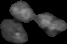
\includegraphics[width=0.18\textwidth]{images/gmm/gmm_2d_fit/t=75,id=446,k=3_raw.png}} &
    \raisebox{\tablemathtext-\height}{
        
\includegraphics[width=0.18\textwidth]{images/gmm/gmm_2d_fit/t=75,id=446,k=3_label.png}} &
    \raisebox{\tablemathtext-\height}{
        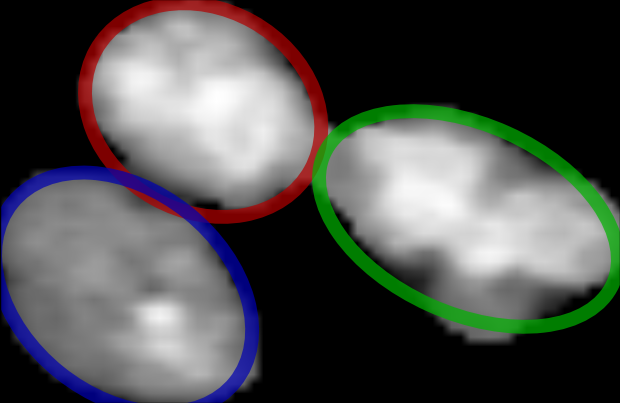
\includegraphics[width=0.18\textwidth]{images/gmm/gmm_2d_fit/t=75,id=446,k=3_fit.png}} \\
    &&& \\
    $t=85$, $\id=12$&
    \raisebox{\tablemathtext-\height}{
        
\includegraphics[width=0.18\textwidth]{images/gmm/gmm_2d_fit/t=85,id=12,k=3_raw.png}} &
    \raisebox{\tablemathtext-\height}{
        
\includegraphics[width=0.18\textwidth]{images/gmm/gmm_2d_fit/t=85,id=12,k=3_label.png}} &
    \raisebox{\tablemathtext-\height}{
        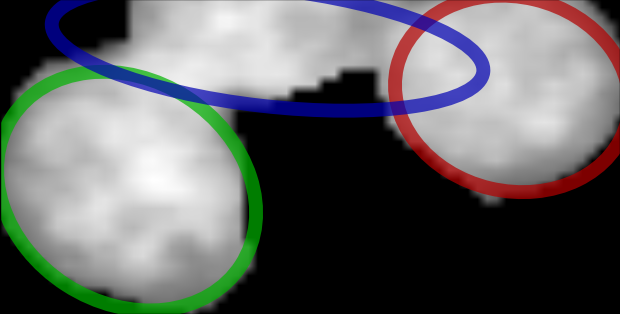
\includegraphics[width=0.18\textwidth]{images/gmm/gmm_2d_fit/t=85,id=12,k=3_fit.png}} \\
    &&& \\
    $t=75$, $\id=206$&
    \raisebox{\tablemathtext-\height}{
        
\includegraphics[width=0.18\textwidth]{images/gmm/gmm_2d_fit/t=75,id=206,k=2_raw.png}} &
    \raisebox{\tablemathtext-\height}{
        
\includegraphics[width=0.18\textwidth]{images/gmm/gmm_2d_fit/t=75,id=206,k=2_label.png}} &
    \raisebox{\tablemathtext-\height}{
        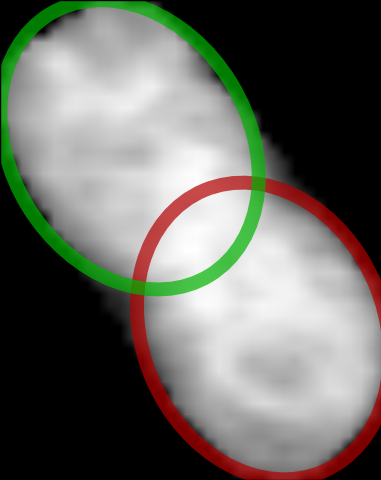
\includegraphics[width=0.18\textwidth]{images/gmm/gmm_2d_fit/t=75,id=206,k=2_fit.png}} \\
    % &
    % \raisebox{\tablemathtext-\height}{
\includegraphics[width=0.18\textwidth]{images/gmm/gmm_2d_fit/t=50,id=198,k=3_raw.png}} &
    % \raisebox{\tablemathtext-\height}{
\includegraphics[width=0.18\textwidth]{images/gmm/gmm_2d_fit/t=50,id=198,k=3_label.png}} &
    % \raisebox{\tablemathtext-\height}{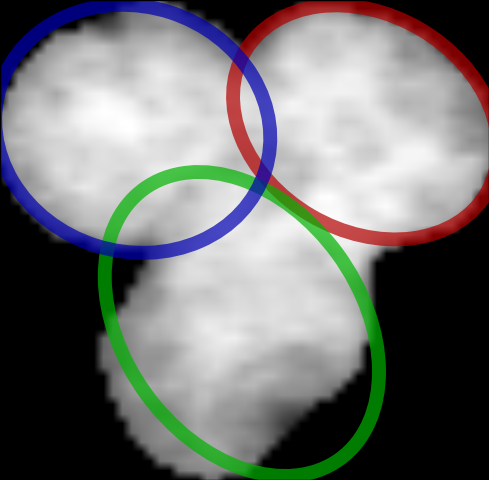
\includegraphics[width=0.18\textwidth]{images/gmm/gmm_2d_fit/t=50,id=198,k=3_fit.png}} \\ &
    &&& \\
    $t=75$, $\id=446$&
    \raisebox{\tablemathtext-\height}{
        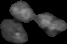
\includegraphics[width=0.18\textwidth]{images/gmm/gmm_2d_fit/t=75,id=446,k=3_raw.png}} &
    \raisebox{\tablemathtext-\height}{
\includegraphics[width=0.18\textwidth]{images/gmm/gmm_2d_fit/t=75,id=446,k=3_label.png}} &
    \raisebox{\tablemathtext-\height}{
        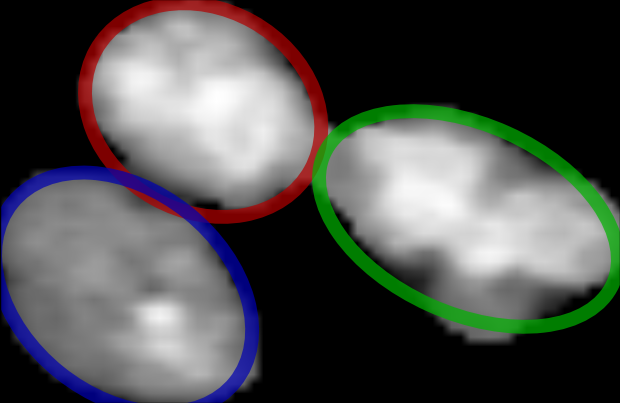
\includegraphics[width=0.18\textwidth]{images/gmm/gmm_2d_fit/t=75,id=446,k=3_fit.png}} \\
    &&& \\
    $t=50$, $\id=122$&
    \raisebox{\tablemathtext-\height}{
        
\includegraphics[width=0.18\textwidth]{images/gmm/gmm_2d_fit/t=50,id=122,k=2_raw.png}} &
    \raisebox{\tablemathtext-\height}{
\includegraphics[width=0.18\textwidth]{images/gmm/gmm_2d_fit/t=50,id=122,k=2_label.png}} &
    \raisebox{\tablemathtext-\height}{
        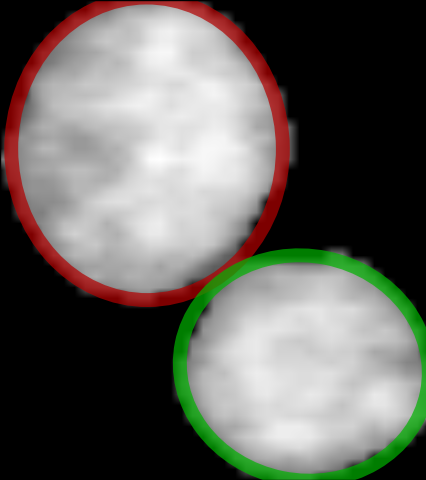
\includegraphics[width=0.18\textwidth]{images/gmm/gmm_2d_fit/t=50,id=122,k=2_fit.png}} \\
    &&& \\
    $t=85$, $\id=334$&
    \raisebox{\tablemathtext-\height}{
        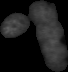
\includegraphics[width=0.18\textwidth]{images/gmm/gmm_2d_fit/t=85,id=334,k=4_raw.png}} &
    \raisebox{\tablemathtext-\height}{
        \hspace{-3pt}
\includegraphics[width=0.18\textwidth]{images/gmm/gmm_2d_fit/t=85,id=334,k=4_label.png}} &
    \raisebox{\tablemathtext-\height}{
        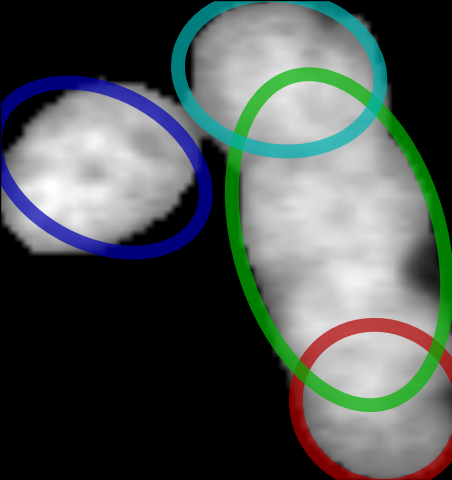
\includegraphics[width=0.18\textwidth]{images/gmm/gmm_2d_fit/t=85,id=334,k=4_fit.png}} \\
    \bottomrule
\end{tabular}
\def\arraystretch{1.0}

% WHY THE FUCK THE NEED FOR NEGATIVE HSPACE IN LAST ROW?

%%% Local Variables: 
%%% mode: latex
%%% TeX-master: "../../../../main"
%%% End: 
